\documentclass[11pt,a4paper]{ctexart}
\usepackage[margin=2.4cm]{geometry}
\usepackage{amsmath}
\usepackage{amssymb}
\usepackage{graphicx}
\usepackage{booktabs}
\usepackage{xcolor}
\usepackage{hyperref}
\hypersetup{
  colorlinks=true,
  linkcolor=black,
  urlcolor=blue,
  pdfborder={0 0 0}
}
% 函数图默认宽度
\newcommand{\plotwidth}{0.4\textwidth}
% 行内代码样式
\newcommand{\incode}[1]{\texttt{\small #1}}

\title{}
\date{}
\begin{document}

\section{三角函数与单位圆}
这是一份示例文档，演示 \textbf{mathtext2doc} 工具的解析能力。文档同时包含中文、 基础 Markdown、LaTeX 公式和 @plot 绘图指令。

\subsection{一、基础公式}
欧拉公式描述了指数函数与三角函数之间的关系：

\begin{equation*}
e^{i\pi} + 1 = 0
\end{equation*}

它是数学中最优雅的等式之一，把五个基本常数 $e$、$i$、$\pi$、$1$、$0$ 联系在一起。

\subsection{二、三角函数图像}
下面同时绘制 $\sin(x)$ 与 $\cos(x)$ 在 $[-\pi, \pi]$ 上的图像：

\begin{figure}[h]
\centering
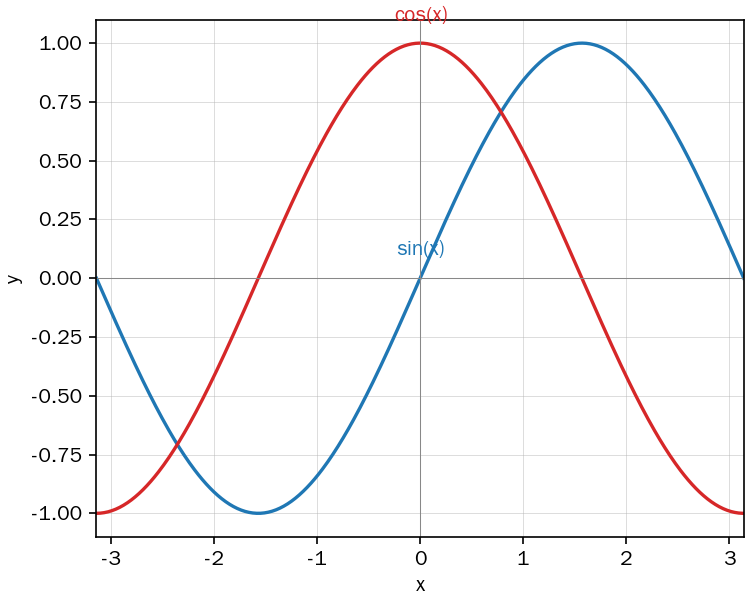
\includegraphics[width=\plotwidth]{sample_input-plot1.png}
\end{figure}

可以看到：

\begin{itemize}
\item 两个函数周期都是 $2\pi$
\item 在 $x=0$ 处 $\sin(0)=0$、$\cos(0)=1$
\item 它们相差 $\pi/2$ 的相位
\end{itemize}

\subsection{三、单位圆}
单位圆是隐函数 $x^2 + y^2 = 1$ 的几何表示：

\begin{figure}[h]
\centering
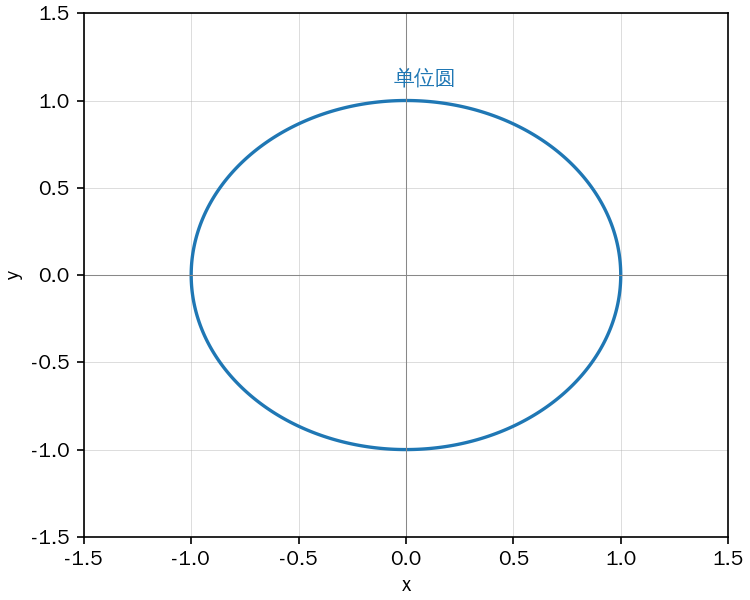
\includegraphics[width=\plotwidth]{sample_input-plot2.png}
\end{figure}

\subsection{四、混合示例}
把显函数和隐函数画在同一张图上：

\begin{figure}[h]
\centering
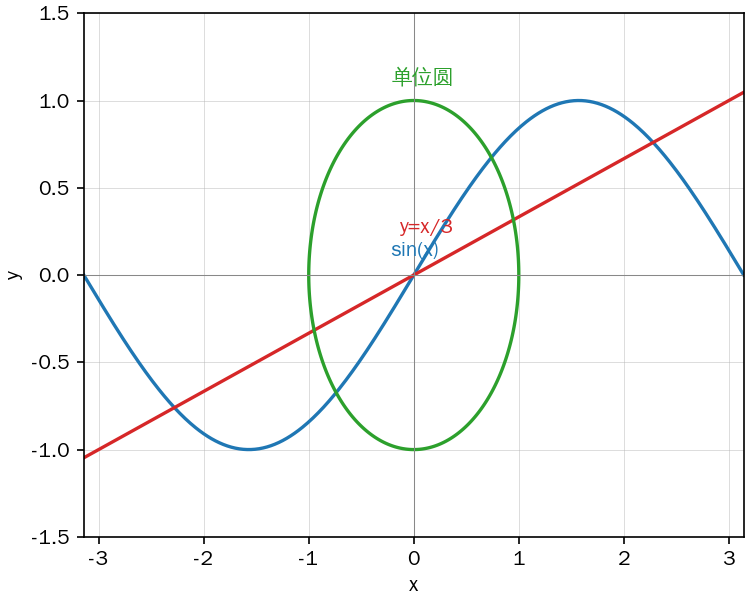
\includegraphics[width=\plotwidth]{sample_input-plot3.png}
\end{figure}

\subsection{五、参数对比表}
\begin{center}
\begin{tabular}{llll}
\toprule
函数 & 定义域 & 值域 & 周期 \\
\midrule
$\sin(x)$ & $\mathbb{R}$ & $[-1, 1]$ & $2\pi$ \\
$\cos(x)$ & $\mathbb{R}$ & $[-1, 1]$ & $2\pi$ \\
$\tan(x)$ & $x \neq \pi/2 + k\pi$ & $\mathbb{R}$ & $\pi$ \\
\bottomrule
\end{tabular}
\end{center}

\end{document}
